\scanpage{6}
\mspage{\textcircled{2}}
% archive foliation: 5
\diagram{\left.\begin{array}{c}A^\circ,\widehat A^\circ,A^\vee\\B^\circ,\widehat B^\circ,B^\vee\end{array}\right|
\begin{tikzcd}[column sep=small,row sep=small]{}\arrow[dr]&{}\\{}\arrow[ur]&{}\end{tikzcd}
\left|\begin{array}{c}\widehat A\\\widehat B\end{array}\right.}\quad(6\text{ Cas})
\[
\left|\widehat A^\circ\ \underset{\unsure{\rightarrow}}{\text{ou}}\ A^\vee\right|
\times\left|\widehat B^\circ\ \text{ou}\ B^\vee\right|\longrightarrow\mathrm{Ens}
\qquad(4\text{ Cas})
\]
\uline{NB}
\diagram{\begin{tikzcd}[row sep=small]
\widehat A^{\circ\unsure{-}}&&A^\vee\\
&A^\circ\arrow[ul,hook]\arrow[ur,hook]&
\end{tikzcd}}
\diagram{\begin{tikzcd}[row sep=small]
\widehat B^\circ&&B^\vee\\
&B^\circ\arrow[ul,hook]\arrow[ur,hook]&
\end{tikzcd}}

\margin{$(\widehat B\rightarrow)$}
\margin{\figure{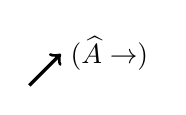
\begin{tikzpicture}\draw[->,very thick](0,0)--(.4,.4);\node[anchor=west] at (.4,.4){$(\widehat A\rightarrow)$};\end{tikzpicture}}}
\diagram{\begin{tikzcd}[column sep=small,row sep=large]
&&&\underline{\mathrm{Hom}}^{!!}(\widehat A^\circ,\widehat B^\circ;\mathrm{Ens})&&&\\
&\underline{\mathrm{Hom}}^!(\widehat B^\circ,\widehat A)\arrow[urr,bend left=15]\arrow[ddl,bend right=15]&&&&\underline{\mathrm{Hom}}^!(\widehat A^\circ,\widehat B)\arrow[ull,bend right=15]\arrow[ddr,bend left=15]\arrow[dl] &\\
&&\underline{\mathrm{Hom}}(B^\circ,\widehat A)\arrow[ul]&&\underline{\mathrm{Hom}}(A^\circ,\widehat B)&&\\
\underline{\mathrm{Hom}}_!^!(A^\vee,\widehat B^\circ;\mathrm{Ens})&&&
\begin{gathered}(A\times B)^\wedge\\=\underline{\mathrm{Hom}}(A^\circ,B^\circ;\mathrm{Ens})\end{gathered}
\arrow[ul]\arrow[ur]\arrow[dl]\arrow[dr]
\arrow[uuu,no head,"\wedge\wedge" description]
\arrow[lll,no head,"\vee\wedge" description]
\arrow[rrr,no head,"\wedge\vee" description]
\arrow[ddd,no head,"\vee\vee" description]
&&&\underline{\mathrm{Hom}}^!_!(\widehat A^\circ,B^\vee;\mathrm{Ens})\\
&&\underline{\mathrm{Hom}}(A^\circ,\widehat B)\arrow[dl]&&\underline{\mathrm{Hom}}(B^\circ,\widehat A)\arrow[dr]&&\\
&\underline{\mathrm{Hom}}_!(A^\vee,\widehat B)\arrow[uul,bend left=15]\arrow[drr,bend right=15]&&&&\underline{\mathrm{Hom}}_!(B^\vee,\widehat A)\arrow[uur,bend right=15]\arrow[dll,bend left=15]&\\
&&&\underline{\mathrm{Hom}}_{!!}(A^\vee,B^\vee;\mathrm{Ens})&&&
\end{tikzcd}}
\margin{$(A^\vee\rightarrow)$\qquad$(B^\vee\rightarrow)$}
Toutes les flèches du diagramme sont des équivalences de catégories

$I$ ens d'indices

$(A_i)_{i\in I}$ famille de (petites) catégories
\figure{\begin{tikzpicture}\draw (0,0)--(0,1.4);\end{tikzpicture}}

Si $I'\subset I$, on pose
\[
A_{I'}=\prod_{i'\in I'}A_{i'}
\]
\[
I=\coprod_{j\in J}I_j,\quad J=J^+\amalg J^-\qquad
I^+=\coprod_{j\in J^+}I_{j^+},\quad I^-=\coprod_{j\in J^-}I_{j^-}
\]
Je suppose $I,J$ finis pour ``play safe''.
\figure{\begin{tikzpicture}\draw(0,0)--(3,1.5);\end{tikzpicture}}
\diagram{\begin{tikzcd}[column sep=large,row sep=large]
&\widehat A_I\arrow[d,"\unsure{\varphi}"',"\simeq"]&\\
&\underline{\mathrm{Hom}}^{\deleted{\unsure{!}}!}_!\left(
\prod_{j^-\in J^-}A_{I_{j^-}}^\vee,
\prod_{j^+\in J^+}A_{I_{j^+}}^{\wedge\circ};\mathrm{Ens}\right)
\arrow[dl,"\approx"']\arrow[dr,"\approx"]&\\
\underline{\mathrm{Hom}}_!\left(\prod_{j^-\in J^-}A_{I_{j^-}}^\vee,\widehat A_{I^+}\right)
&&\underline{\mathrm{Hom}}^!\left(\prod_{j^+\in J^+}A_{I_{j^+}}^{\wedge\circ},\widehat A_{I^-}\right)
\end{tikzcd}}
